\documentclass[10pt, twocolumn]{article}
\usepackage[margin=1in]{geometry}
\usepackage{lmodern}% http://ctan.org/pkg/lm
\usepackage{authblk} % adds affiliations

\usepackage[utf8x]{inputenc}
\usepackage{nameref}
\usepackage[switch]{lineno}
\usepackage{amsmath}
\usepackage{booktabs}
\usepackage[numbers,super]{natbib}
\usepackage{changepage}

% adjust caption style
\usepackage[aboveskip=1pt,labelfont=bf,
            labelsep=period,singlelinecheck=off]{caption}

% remove brackets from references
\makeatletter
\renewcommand{\@biblabel}[1]{\quad#1.}
\makeatother

\usepackage[colorinlistoftodos]{todonotes}

% headrule, footrule and page numbers
\usepackage{lastpage,fancyhdr,graphicx}
\usepackage{epstopdf}
\pagestyle{myheadings}
\pagestyle{fancy}
\fancyhf{}
\rfoot{\thepage/\pageref{LastPage}}
\renewcommand{\footrule}{\hrule height 2pt \vspace{2mm}}

% use \textcolor{color}{text} for colored text (e.g. highlight to-do areas)
\usepackage{color}

\definecolor{Gray}{gray}{.25}

\usepackage{graphicx}

% use if you want to put caption to the side of the figure
\usepackage{sidecap}

\usepackage{xcolor}
\usepackage[colorlinks = true,
            linkcolor = blue,
            urlcolor  = blue,
            citecolor = blue,
            anchorcolor = blue]{hyperref}

% ####################################################
% ####################################################
\usepackage[colorinlistoftodos]{todonotes}
% ####################################################
% ####################################################

% use for have text wrap around figures
\usepackage{wrapfig}
\usepackage[pscoord]{eso-pic}
\usepackage[fulladjust]{marginnote}
\reversemarginpar{}

\usepackage{gensymb}
\usepackage{siunitx}

% make a box for author summary
\usepackage[framemethod=TikZ]{mdframed}
%% define the style
\newcommand{\mybox}[2]{%
         \begin{center}%
            \begin{tikzpicture}%
                \node[rectangle, draw=#1, top color=#1!10, bottom color=#1!10,
                      rounded corners=5pt, inner xsep=5pt, inner ysep=6pt,
                      outer ysep=10pt]{
                        \begin{minipage}{1\textwidth}#2\end{minipage}};%
            \end{tikzpicture}%
         \end{center}%
}

% new commands
% q value
\newcommand{\qval}[1]{$q<10^{-#1}$}

% species names
\newcommand{\cel}{\emph{C.~elegans}}
\newcommand{\dicty}{\emph{D.~discoideum}}
\newcommand{\ecol}{\emph{E.~coli}}
\newcommand{\gf}{gain-of-function allele}
\newcommand{\lf}{loss-of-function allele}
\newcommand{\strong}{strong loss-of-function allele}
\newcommand{\weak}{weak loss-of-function allele}

% gene names
% \newcommand{\gene}[1]{\emph{#1}} # for MS word typesetting
\newcommand{\gene}[1]{\mbox{\emph{#1}}}
\newcommand{\genotype}[1]{\mbox{\emph{#1}}}
\newcommand{\protein}[1]{\mbox{\uppercase{#1}}}
\newcommand{\ras}{\gene{let-60} (\emph{ras})}
\newcommand{\rasp}{\protein{let-60}}
\newcommand{\dpy}{\gene{dpy-22} (\emph{MED-12})}
\newcommand{\letgfn}{3,021}
\newcommand{\letlfn}{857}
\newcommand{\letgf}{\gene{let-60(gf)}}
\newcommand{\letlf}{\gene{let-60(lf)}}
\newcommand{\strongn}{2,821}
\newcommand{\weakn}{434}
\newcommand{\transn}{2,930}


% more space between rows
\newcommand{\ra}[1]{\renewcommand{\arraystretch}{#1}}

\title{A study of allelic series using transcriptomic phenotypes}

\author[1,2]{David Angeles-Albores}
\author[1,2,*]{Paul W. Sternberg}
\affil[1]{Division of Biology and Biological Engineering, Caltech,
Pasadena, CA, 91125, USA}
\affil[2]{Howard Hughes Medical Institute, Caltech, Pasadena, CA, 91125, USA}
\affil[*]{Corresponding author. Contact: pws@caltech.edu}
\renewcommand\Affilfont{\itshape\small{}}

% document begins here
\begin{document}
% title

\twocolumn[
  \begin{@twocolumnfalse}
    \maketitle
    % \section*{Abstract}
    \textbf{Expression profiling holds great promise for genetics due to
    its quantitative nature and the large number of genes that are measured. There
    is increasing interest in using these measurements as phenotypes for classical
    genetics analysis. Although transcriptomes have recently been used to perform
    epistasis analyses for pathway reconstruction, there has not been a systematic
    effort to understand whether different alleles have different transcriptomic
    qualities. Here, we study two allelic series using transcriptomic phenotypes. We
    studied two alleles of \gene{dpy-22}
    that generate prematurely truncated proteins of different lengths. We show
    that expression perturbations caused by these alleles can be split into three
    distinct modules, and each module reacts with a different dominance relationship
    to each allele. Our work formalizes the concept of dominance for transcriptomic
    phenotypes, and shows the importance of studying allelic series for
    understanding the molecular qualities of the genes in question.
    }
    \vspace{5mm}

    \mybox{red}{
    \section*{Author Summary}
    Expression profiling is a way to quickly and quantitatively measure the expression
    level of every gene in an organism. As a result, these profiles could be used as
    phenotypes with which to perform genetic analyses (i.e., to figure out what genes
    interact with each other) as well as to dissect the molecular properties of each
    gene. Before we can perform these analyses, we have to figure out the rules that
    apply to these measurements. In this paper, we develop new concepts and methods
    with which to study an allelic series. Briefly, allelic series are an important
    aspect of genetics because different alleles encode different versions of a gene.
    By studying these different versions, we can make statements about the function
    of different parts of the gene. By combining allelic series with expression
    profiling, we can learn much more about the gene under study than we could
    previously.
    }
    \vspace{5mm}
  \end{@twocolumnfalse}
]


\linenumbers{}

\section*{Introduction}
The term `allelic series' refers to the study of alleles with different
phenotypes to understand the molecular properties that this locus controls.
Allelic series are historically important for genetics. The earliest
Pubmed-indexed author to use this term was Barbara
McClintock~\cite{McClintock1944}. In her work, McClintock studied a deficiency
of the tail end of chromosome 9 of maize by generating \emph{trans}-heterozygotes with
mutants of various genes that she knew existed near the end of chromosome 9. Her
work allowed her to infer that the deficiency was modular, effectively
generating a double mutant that behaved as a single allele but which could
participate phenotypically in two distinct allelic series. From this study,
McClintock inferred that deletions could span multiple genes, which behaved
as independent modules, and which were identified via complementation assays.
This work set the foundations for later observations in yeast
that showed two mutant alleles of the same genetic unit, when placed in
\emph{trans} to each other, could complement and generate a wild-type
phenotype~\cite{FINCHAM1957}. Allelic series have also been used to study the
dose response curve of a phenotype for a particular gene. In \cel{}, the
\gene{let-23} allelic series stands out as such an example~\cite{}.

Over the last decade, biology has moved from studies of single genes towards
studies of genome-wide measurements. In particular, expression profiling via
RNA-sequencing~\cite{Mortazavi2008} (RNA-seq) is a popular method because it
enables the simultaneous measurement of expression levels for all genes in a
genome. These measurements can now be made on a whole-organism scale and on
single cells~\cite{Tang2009}. Although initially expression profiles had a
qualitative purpose as descriptive methods to identify genes that are downstream
of a perturbation, these profiles are now being used as phenotypes for genetic
analysis. As a result, transcriptomes have been successfully used to identify
new cell or organismal states~\cite{Angeles-Albores2017,Villani2017}. Genetic
pathways have been reconstructed via sequencing single cells~\cite{Dixit2016} or
by sequencing whole-organisms~\cite{}. However, to fully characterize a genetic
pathway, it is often necessary to build allelic series to compare how phenotypes
change with varying gene activity.

As a proof of principle, we selected a subunit of the Mediator complex in
\cel{}, \gene{dpy-22} (also known as \gene{mdt-12}), for genetic analysis.
Mediator is a macromolecular complex that contains 25 or so
subunits~\cite{Jeronimo2017} and which globally regulates RNA polymerase II (Pol
II)~\cite{Allen2015,Takagi2006}. Mediator is a versatile regulator, a quality
often associated with its variable subunit composition~\cite{Allen2015}, and it
can promote transcription as well as inhibit it. The Mediator complex consists
of four modules: the Head, Middle and Tail modules and a CDK-8-associated
Kinase Module (CKM). The CKM
can associate reversibly with Mediator. Certain models propose that the CKM
functions as a molecular switch, which inhibits Pol II activity by sterically
preventing its interaction with the other Mediator
modules~\cite{Knuesel2009,Elmlund2006}. Other models propose that the CKM
negatively modulates interactions between Mediator and
enhancers~\cite{VandePeppel2005}. In \cel{}, the CKM
consists of \protein{cdk-8}, \protein{mdt-13}, \protein{cic-1} and
\protein{DPY-22}~\cite{Grants2015}. Since \gene{dpy-22} is orthologous
to the human Mediator subunits \gene{MED-12} and \gene{MED-12L}~\cite{Zhang2000},
we will henceforth refer to this gene as \dpy{}.
\todo[inline]{dpy-22 in gene dosage sentence?}
\dpy{} has been studied in the context of the male tail~\cite{Zhang2000}, where
it was found to interact with the Wnt pathway. It has also been studied in
the context of vulval formation~\cite{Moghal2003a}, where it was found to be an
inhibitor of the Ras pathway. \dpy{} is likely an essential gene, and
developmental studies have relied on reduction-of-function alleles to understand
the role of this gene in development. Studies of the male tail were carried out
using an allele, \gene{dpy-22(bx93)}, that generates a truncated
\protein{dpy-22} protein missing its C-terminal 900 or so amino
acids as a result of a premature stop codon, Q2549STOP~\cite{Zhang2000}. In
spite of the premature truncation, animals carrying this allele grossly appear
phenotypically wild-type. In contrast, the allele used to study the role of
\dpy{} in the vulva, \gene{dpy-22(sy622)}, is a premature stop codon, Q1689STOP,
that predicted to remove over 1,500 amino acids from the
C-terminus~\cite{Moghal2003}. Animals carrying this mutation are severely dumpy
(Dpy), have egg-laying defects (Egl) and have a multivulva (Muv) phenotype that
occurs at a very low rate (see Fig.~\ref{fig:dpy22}). We wanted to study how
truncations of increasing severity affected transcriptomic phenotypes. These
alleles could form a single quantitative series, affecting the same sets of
target genes but to different degrees, in which case the
\emph{trans}-heterozygote would exhibit a single dosage-dependent phenotype
intermediate to the two homozygotes. Alternatively, they could form a single
qualitative series, in which case the \emph{trans}-heterozygote should have the same
phenotype as the homozygote of the \emph{bx93} allele, since this allele encodes
the longer protein. These alleles could also form a mixed series, in
which case multiple separable phenotypes would appear that have qualitative or
quantitative behaviors in the \emph{trans}-heterozygote.

\begin{figure}
  \centering{}
  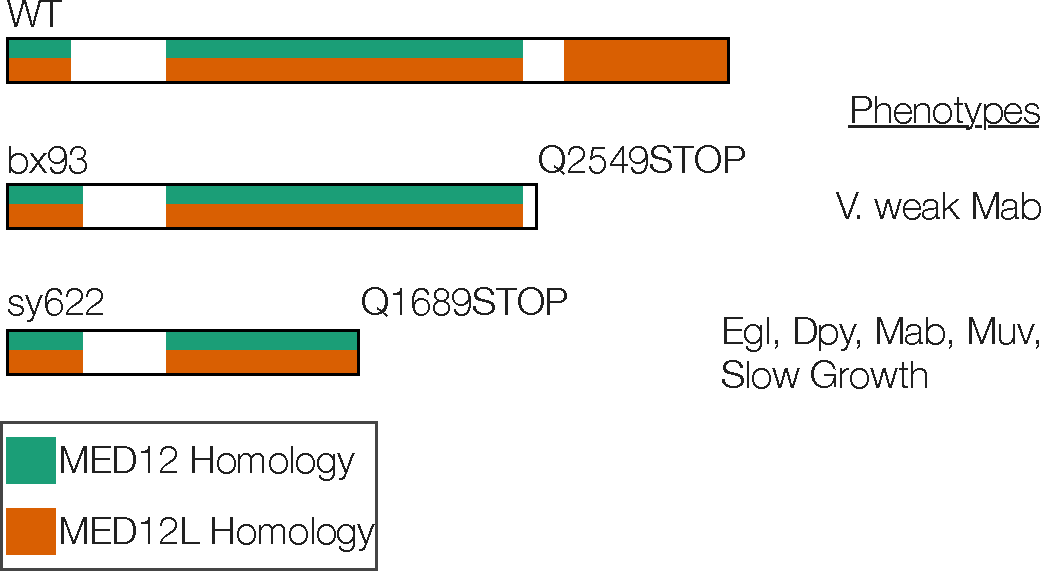
\includegraphics[width=0.5\textwidth]{../figs/gene_model_dpy22.pdf}
  \caption{
    The \dpy{} allelic series, consisting of two amino acid truncations,
    is amenable to study by transcriptomic phenotypes. Diagram of
    the \dpy{} gene and the \emph{bx93} and \emph{sy622} alleles. Conservation
    between \dpy{} and its human orthologs is shown in color.
    }
\label{fig:dpy22}
\end{figure}

Expression profiles have the potential to facilitate
dissection of molecular structures within genes. To establish a methodology for
studying allelic series, we explored three alleles (including the wild-type
allele) of the highly pleiotropic gene, \dpy{}. For the \dpy{} allelic series, we
found that the perturbations caused by the weak loss-of-function allele,
\emph{bx93}, are entirely contained within the strong loss-of-function allele,
\emph{sy622}. Further, we found that there are three phenotypic classes that are
affected by \dpy{}. For one class, termed the \emph{sy622}-specific class, the
\emph{bx93} homozygote, but not the \emph{sy622} homozygote, shows wild-type
functionality. In a \emph{trans}-heterozygote of \emph{sy622/bx93} these genes are
suppressed to wild-type levels from the \emph{sy622} levels, which shows that
\emph{bx93} is wild-type dominant for this phenotype. A second class, called the
\emph{sy622}-associated class, similarly shows wild-type functionality in the
\emph{bx93} homozygote but not in the \emph{sy622} homozygote, yet in the
\emph{trans}-heterozygote the expression levels of these genes is modulated in a
gene-dosage dependent manner. Finally, we identified a third class, called the
\emph{bx93}-specific class, which contained genes that were altered in both
homozygotes, but which showed an expression level most similar to the
\emph{bx93} homozygote, showing that \emph{bx93} has a dominant mutant phenotype
for this subset. For each class, we were able to quantitatively measure the
dominance level of each allele.


\section*{Results}

\subsection*{A strong and a weak loss-of-function \gene{dpy-22} allele show
             different transcriptomic profiles}
% Previous studies suggested that two alleles of \dpy{}, \emph{sy622} and \emph{bx93},
% might be qualitatively different~\cite{Moghal2003}. Allele
% \emph{bx93} encodes a premature stop codon that removes the terminal 900 amino
% acids from the protein. \emph{bx93} homozygotic animals are phenotypically grossly
% wild-type with a very low incidence of male tail defects~\cite{Zhang2000}. Allele
% \emph{sy622} encodes a premature stop codon that removes the
% terminal 1700 amino acids from the protein. \emph{sy622} homozygotes grow
% slowly, are severely dumpy (Dpy), have a low penetrance multivulva (Muv) phenotype
% and have a prominent egg-laying defective (Egl) phenotype~\cite{Moghal2003}.

% TODO:insert methods nameref here
We sequenced in triplicate mRNA extracted from \emph{sy622} homozygotes,
\emph{bx93} homozygote, a
\emph{trans}-heterozygote of both alleles and a wild-type control at a depth of
20 million reads. This allowed us to identify 21,954 protein-coding isoforms. We
calculated differential expression with respect to a wild-type control using a
general linear model (see~\nameref{sec:methods}). Differential expression with
respect to the wild-type control for each transcript $i$ in a genotype $g$ is
measured via a coefficient $\beta_{g, i}$, which can be loosely interpreted as
the natural logarithm of the fold-change. Positive $\beta$ coefficients indicate
up-regulation with respect to the wild-type, whereas negative coefficients
indicate down-regulation. Transcripts were considered to have differential
expression between wild-type and a mutant if the associated $q$-value of the
$\beta$ coefficient was less than 0.1.

Using these definitions, we found \weakn{} differentially expressed
genes in the  \emph{bx93} homozygote transcriptome, and \strongn{}
differentially expressed genes in the \emph{sy622} homozygote transcriptome. The
\emph{trans}-heterozygote transcriptome had \transn{} differentially expressed
genes.

\subsection*{The transcriptome of a \emph{trans}-heterozygote of \gene{dpy-22}
             identifies four phenotypic classes}
% TODO: check numbers here
We sequenced a \emph{trans}-heterozygote of the \emph{bx93} and \emph{sy622}
alleles with genotype \gene{dpy-6(e14) bx93/+ sy622}. This
\emph{trans}-heterozygote appears phenotypically wild-type, resembling the
\emph{bx93} mutant morphologically~\cite{Moghal2003}. Using the
\emph{trans}-heterozygote, we identified five non-overlapping phenotypic classes
by what genotypes caused these genes to become differentially expressed (see
Fig.~\ref{fig:venn}). We called the set of genes that were differentially
expressed only in the \emph{bx93} homozygote relative to the wild type the
\emph{bx93}-specific phenotypic class. We do not analyze this class further due
to its small size (43 genes; see~\nameref{sec:conclusions}). Next, we defined
the set of 296 genes that were differentially expressed in the \emph{bx93}
homozygote and at least one other genotype as the \emph{bx93}-associated
phenotypic class. The \emph{sy622}-associated phenotypic class, which consisted
of 825 genes, was defined as the set of genes that were differentially expressed
in the \emph{sy622} homozygote and in the \emph{trans}-heterozygote, but which
did not already belong to the \emph{bx93}-associated phenotypic class. The
\emph{sy622}-specific phenotypic class (1,477 genes) and the
\emph{trans}-heterozygote-specific phenotypic classes (1,536 genes) were defined
as the sets of genes that were only differentially expressed in each genotype.
Having defined these phenotypic classes, we set out to confirm whether each
class actually behaved as an independent phenotypic module in an allelic series
and whether each class could be interpreted biologically to shed light on the
structure of \dpy{}.


\begin{figure}
  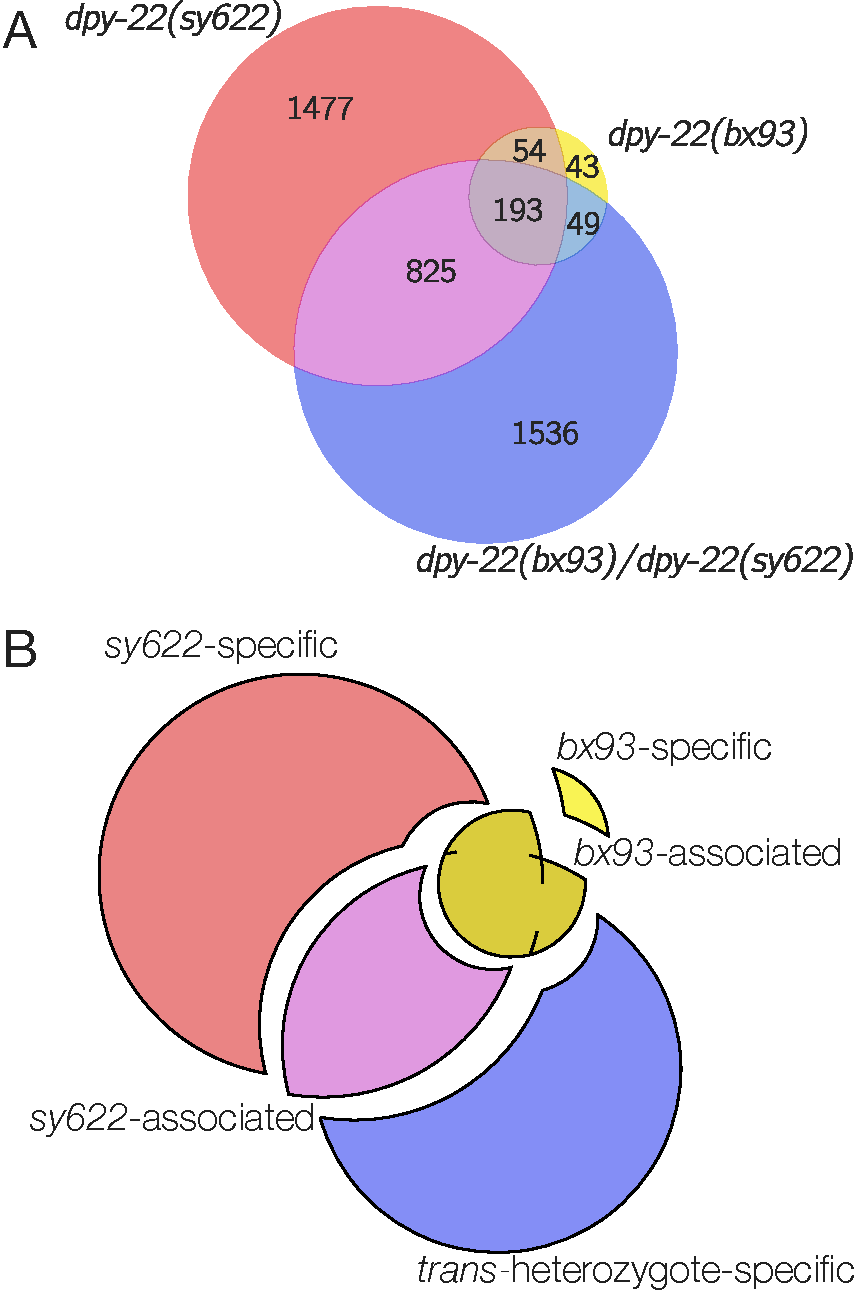
\includegraphics[width=0.5\textwidth]{../figs/venn_diagrams.pdf}
  \caption{
  Transcripts under the control of \dpy{} belong to distinct phenotypic
  classes.
  \textbf{A} Venn diagram showing number of genes in each subset.
  \textbf{B} Exploded Venn diagram highlighting the five identified phenotypic
  classes.
  }
\label{fig:venn}
\end{figure}

\subsection*{Different phenotypic classes behave differently in an
            \emph{sy622} homozygote}
We asked whether these classes had perturbation distributions distinct from each
other within a single homozygote. Specifically, in the context of the
\emph{sy622} homozygote, we wanted to know whether the \emph{sy622}-specific,
the \emph{sy622}-associated and the \emph{bx93}-associated phenotypes were
different in the magnitude of their perturbations or whether these subsets
behaved as if they had been randomly selected from the set of differentially
expressed genes in the \emph{sy622} homozygote, in which case the distributions
of effects would be the same for all classes (see Fig.~\ref{fig:classes}). We
found that that the $\beta$ coefficients of isoforms within the
\emph{bx93}-associated phenotype on average had the largest absolute value (mean
$1.3$). The \emph{sy622}-associated phenotype had a smaller range of
perturbations compared to the \emph{bx93}-associated phenotype (95th percentiles
of the two distributions: 3.6 versus 4.1, respectively), and a statistically
smaller mean (1.1 vs 1.3, respectively, $p = 1.7 \cdot 10^{-5}$, non-parametric
boostrap). The \emph{sy622}-specific phenotype had the smallest mean of all
(0.95, $p < 10^{-6}$ compared with \emph{bx93}-associated phenotype).

% to make figure span two columns in twocolumn mode, use figure*
\begin{figure*}
  \centering{}
  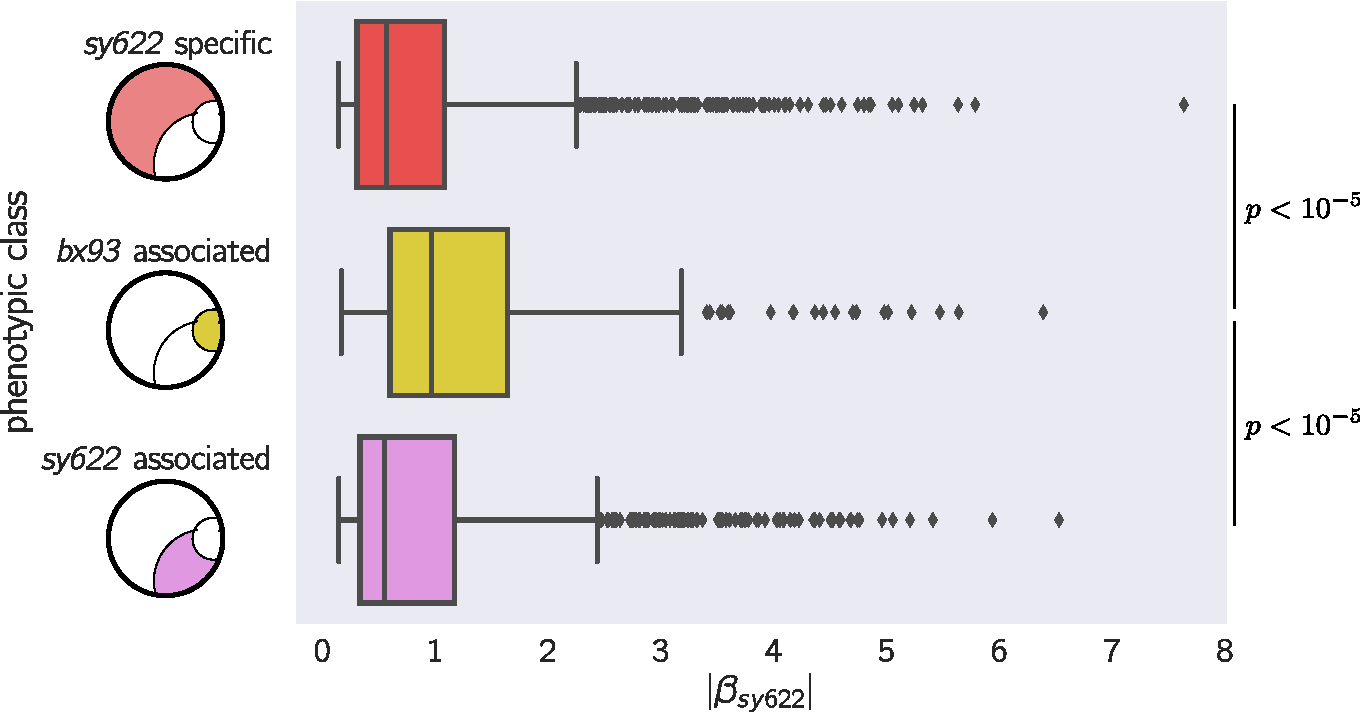
\includegraphics[width=0.75\textwidth]{../figs/dpy22_classes.pdf}
  \caption{
    Within the \emph{sy622} homozygote mutant, different phenotypic classes have
    statistically different distributions. The lines
    within the boxes show the 25, 50, and 75 percentiles. Whiskers show the rest
    of the plot, except for outliers (diamonds). Diagrams show what genotypes each
    gene class is expressed in, but the magnitude of the perturbation plotted
    always corresponds to the \emph{sy622} mutant.
    The medians of the \emph{sy622}-specific and the \emph{sy622}-associated
    classes were statistically significantly different from the mean of the
    \emph{bx93}-specific class, as assessed by a non-parametric bootstrap test.
  }
\label{fig:classes}
\end{figure*}

\subsection*{Dominance can be quantified in transcriptomic phenotypes}
\todo[inline]{quantitative genetics citation?}
We reasoned that if one allele was dominant over the other in the heterozygote,
then plotting the $\beta$ coefficients in the homozygote of the dominant allele
versus the heterozygote should lead to a slope of 1. Deviations from a slope
with magnitude equal to unity should therefore be interpreted as deviations from
a standard dominant-recessive model. When expression in a \emph{trans}-heterozygote
is intermediate between the two homozygotes, this suggests a co-dominance regime
where both alleles are contributing to the phenotype in a weighted fashion.

% TODO: Cite let-23 allelic series paper
Dominance relationships between alleles are phenotype-specific. In other
words, an allele can be dominant over another for one phenotype, yet not for
others. An example is the \gene{let-23} allelic series---nulls of
\gene{let-23} are recessive lethal (Let) and presumably also recessive vulvaless
(Vul) relative to the wild-type allele. The \emph{sy1} allele of
\gene{let-23} is viable dominant relative to null alleles, but is recessive
Vul~\cite{} to the wild-type allele. Above, we postulated that there are four
phenotypic classes, three of which are perturbed in the \emph{sy622} homozygote.
If these classes are indeed modular phenotypes, then the dominance relationships
within each class should be the same from gene to gene. In other words, a single
dominance coefficient should be sufficient to explain the gene expression in the
\emph{trans}-heterozygote for every gene within a class.

To quantify this dominance, we implemented and maximized a Bayesian model.
Briefly, we asked what the linear combination of $\beta$ coefficients from each
homozygote would best predict the observed $\beta$ values of the heterozygote,
subject to the constraint that the coefficients added up to 1 (see
\nameref{subsec:dominance}). We reasoned that if this was a modular phenotype
controlled by a single structure encoded within the gene of interest, then a
plot of the predicted $\beta$ values from the optimized model against the
observed $\beta$ values of the heterozygote for each transcript should show the
data falling along a line with slope equal to unity. Systematic deviations from
linear behavior would indicate that the transcripts plotted are not part of a
modular phenotypic class controlled by a single structure.

\subsubsection*{The \emph{sy622}-specific class expression phenotype of the
                \emph{sy622} homozygote is complemented to wild-type levels by
                the presence of a \emph{bx93} allele}
Since our previous testing showed that the transcript expression of genes in
this class was dysregulated in \emph{sy622} homozygotes, and wild-type in both
\emph{bx93} homozygotes and \emph{trans}-heterozygotes we can conclude that
these transcripts are complemented to their wild-type levels by the presence of
the \emph{bx93} allele. Applying the Bayesian model yields identical results.
Thus, there is a module that has wild-type functionality in the \emph{bx93}
allele but is partially or completely deleted in the \emph{sy622} allele. This
functionality must be encoded between amino acid position 1,689, where the
\emph{sy622} allele truncates prematurely, and the position 2,549 where the
\emph{bx93} allele stops.

\subsubsection*{The \emph{bx93} allele is dominant over the \emph{sy622} for the
                \emph{bx93}-associated phenotype}
We explored how expression levels of transcripts within the
\emph{bx93}-associated phenotypic class were controlled by these two alleles.
We first applied our dominance analysis to transcripts in this class. We found
that the \emph{bx93} allele is largely dominant ($d_{bx93}=0.82$) over the \emph{sy622}
allele (see Fig.~\ref{fig:bx93_associated}). A large dominance coefficient might
indicate that, for this phenotypic class, the \emph{bx93} has a functional
structure that is not present in the \emph{sy622} allele. However, a significant
portion of the transcripts within this class are differentially
expressed in both homozygotes studied. Therefore, if this class is
controlled by a single structure, then the functionality of this structure cannot
be intact in the \emph{bx93} homozygote. Moreover, when we compared the expression
levels of transcripts in \emph{sy622} and \emph{bx93} homozygotes, we found that
the \emph{bx93} homozygotes had $\beta$ coefficients that were on average
39\% weaker than in the \emph{sy622} homozygote. This implies that the
two alleles should be codominant to each other, which is at odds with the
dominance coefficient we observed. The mixed evidence precludes a conclusion
about the structure/function relationship underlying this phenotypic class.

\begin{figure}
  \centering{}
  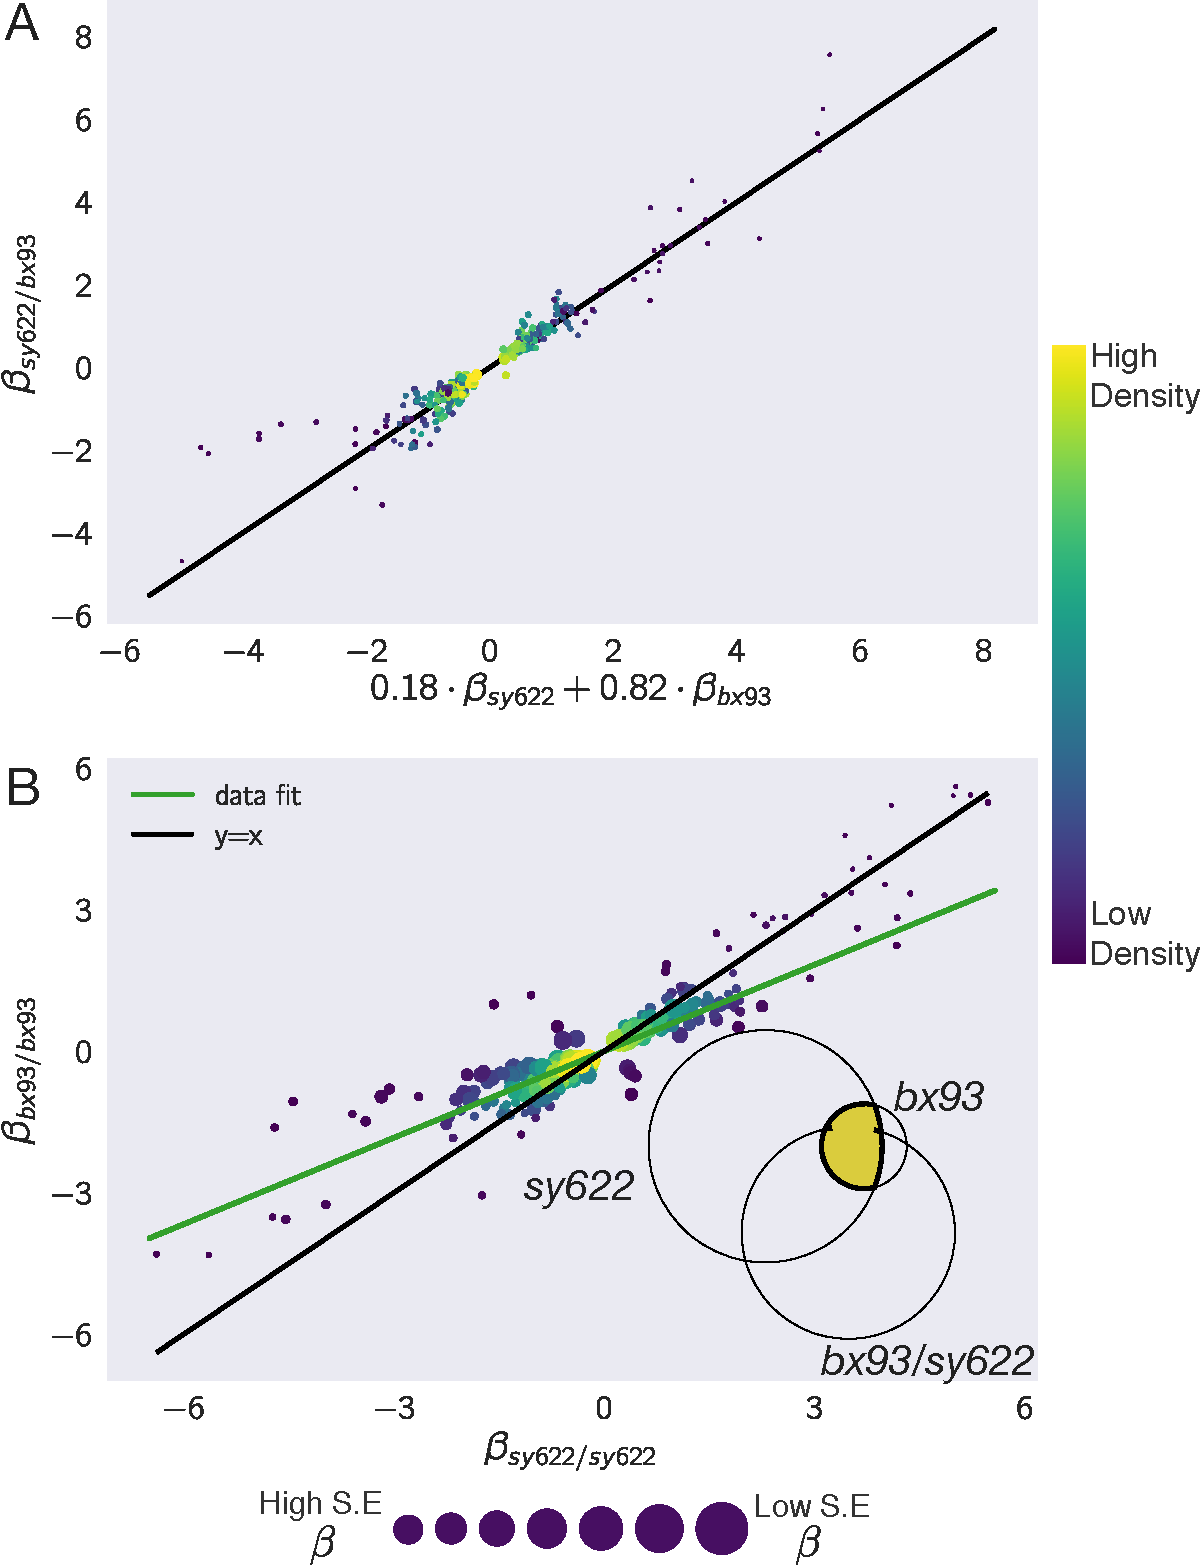
\includegraphics[width=0.5\textwidth]{../figs/bx93_associated_analysis.pdf}
  \caption{The \emph{bx93}-associated class has properties of both quantitative
    and qualitative allelic series.
    \textbf{A} In a \emph{trans}-heterozygote, the \emph{bx93} allele is largely
    dominant over the \emph{sy622} allele for the expression levels of
    transcripts in the \emph{bx93}-associated class.
    \textbf{B} A majority of the transcripts in the \emph{bx93}-associated class
    are differentially expressed in homozygotes of both alleles. In \emph{bx93}
    homozygotes, these transcripts are less perturbed than in \emph{sy622}
    homozygotes.
    }
\label{fig:bx93_associated}
\end{figure}

\subsubsection*{The \emph{sy622}-associated phenotype is attenuated by the presence
            of \emph{bx93} in the \emph{trans}-heterozygote}
We also wanted to know whether the \emph{sy622}-associated phenotype showed
differences depending on genotypic context. We quantified the relative dominance
of \emph{bx93} and \emph{sy622} on the expression level of transcripts of this
class. We found that both alleles are codominant ($d_{bx93} = 0.51$). This
suggests that there is a structure distributed evenly throughout the gene
body starting the first amino acid position and ending before position 2,549
(the site of the \emph{bx93} truncation, otherwise these transcripts would be
differentially expressed in \emph{bx93} homozygotes). Since the two alleles are
co-dominant for transcript expression in this class, the functionality encoded
in this gene must be dosage-dependent for this model to hold.

\subsection*{The \emph{sy622}-specific class is strongly enriched for a Dpy
             transcriptional signature}
\emph{bx93} homozygotic animals are almost wild-type, but careful measurements
show that they have a slight body length defect causing them to be slightly Dpy,
and \emph{sy622} homozygotic animals are known to be severely
Dpy~\cite{Moghal2003}, but this phenotype is complemented almost to wild-type
levels when the \emph{bx93} allele is placed in \emph{trans} to the \emph{sy622}
allele. The only class that is fully complemented to wild-type levels is the
\emph{sy622}-specific class. We hypothesized that the
\emph{sy622}-specific class should show a strong transcriptional Dpy signature.

To test this hypothesis, we derived a Dpy signature from two Dpy mutants
(\gene{dpy-7} and \gene{dpy-10}, \emph{unpublished data}) consisting of 628
genes. We used this gene set to look for a transcriptional Dpy signature in each
phenotypic class using a hypergeometric probabilistic model
(see~\nameref{sec:methods}). We found that the \emph{sy622}-specific and
-associated classes were enriched in genes that are transcriptionally associated
with a Dpy phenotype. The \emph{bx93}-associated class also showed significant
enrichment (fold-change = 2.2, $p=4\cdot10^{-10}$, 68 genes observed). The
enrichment was of considerably greater magnitude in the \emph{sy622}-specific
class (fold-change enrichment = 3, $p=2\cdot 10^{-40}$, $167$ genes observed)
than the enrichment in the \emph{sy622}-associated class (fold-change = 1.9,
$p=9\cdot10^{-9}$, 82 genes observed) or in the \emph{bx93}-associated class.
Correlation analysis showed that a majority of the genes in the
\emph{sy622}-specific class were perfectly correlated between the expression
levels in the Dpy signature and the expression levels in \emph{sy622}
homozygotes, while 25\% of the genes were anti-correlated (Spearman R = 0.42,
$p=6\cdot10^{-15}$). If the anti-correlated values are excluded from the
Spearman regression, the statistical value of the regression improves
significantly (Spearman R = 0.94, $p=2\cdot10^{-108}$). Taken together, this
suggests that the \emph{sy622}-specific phenotypic class contains a
transcriptional signature that can be associated with the morphological Dpy
phenotype.

As a negative control, we also tested a hypoxia dataset, since \emph{dpy-22} is
not known to be associated with the \gene{hif-1}-dependent hypoxia response in
\cel{}. Enrichment tests revealed that the hypoxia response was significantly
enriched in the \emph{bx93}-associated (fold-change = 2.1, $p=10^-{8}$, 63 genes
observed), the \emph{sy622}-associated (fold-change = 1.9, $p=4\cdot10^{-8}$, 78
genes observed) and the \emph{sy622}-specific classes (fold-change = 2.4,
$p=9\cdot10^{-55}$, 186 genes observed). However, correlation analysis revealed
that the expression levels of these genes are not correlated between \dpy{}
mutants and the hypoxia response ($p > 0.4$ in all cases). Therefore, although
genes associated with the hypoxia response are perturbed in \dpy{}
loss-of-function mutants, these genes do not reflect engagement of a
\gene{hif-1}-dependent hypoxia response.

\subsection*{Interactions with the RAS and WNT pathways}




% This suggests that
% the \emph{sy622}-specific class is
% Whereas the \emph{sy622} homozygote is visibly different from the wild type (see
% Fig.~\ref{fig:dpy22}), the \emph{bx93} is almost entirely wild-type. Since the
% \emph{trans}-heterozygote also appears grossly wild-type, we hypothesized that the
% \emph{sy622}-specific phenotypic class was associated with the macroscopic
% phenotypes visible in the \emph{sy622} allele. We used the Wormbase Enrichment
% Suite~\cite{Angeles-Albores2016,Angeles-Albores106369} to query what anatomical,
% phenotypic or gene ontological terms were enriched in each phenotypic class.
%
% The \emph{bx93}-specific gene class returned no enriched anatomy, phenotype
% or gene ontology terms, consistent with our interpretation that this class plays
% a minor role in the biology of \dpy{}. The \emph{trans}-heterozygote specific
% class was enriched in the anatomy terms `male' (Enrichment Fold Change, $FC=2$,
% \qval{40}) and `reproductive system' ($FC=1.3$, \qval{19}), but showed no
% phenotype enrichment. Gene enrichment for this category showed enrichment of many
% terms. Some of the top terms included `cell death' ($FC=3.9$, \qval{28}) and
% `gene silencing by RNA' ($FC=5$, \qval{13}).
%
% The \emph{sy622}-associated class showed enrichment in the intestine ($FC=1.3$,
% \qval{3})
% % , `Psub1' ($FC=2.3$, \qval{2}),  `AB' ($FC=3.0$, \qval{2}) and `cephalic
% % sheath cell' ($FC=2.1$, \qval{2})
% . Phenotype enrichment analysis of this class
% showed
% no enrichment
% % enrichment of the terms `dauer constitutive' ($FC=5.8$, \qval{2}),
% % `cadmium hypersensitive' ($FC=7.3$, \qval{2}) and `pathogen susceptibility'
% % ($FC=4.9$, \qval{2}).
% Gene ontology enrichment analysis identified terms such as
% `oviposition' ($FC=4.1$, \qval{6}), `tube development' ($FC=9.1$, \qval{8}) and
% `collagen trimer' ($FC=4.6$, \qval{4}).
%
% The \emph{sy622}-specific class showed enrichment in the intestine ($FC=1.4$,
% \qval{15}), the muscular system ($FC=1.3$, \qval{7}), the epithelial system
% ($FC=1.2$, \qval{3}) and sex organs ($FC=1.3$, \qval{3}). This class had
% enrichment of terms associated with general sickness and pleiotropy, namely
% `avoids bacterial lawn' ($FC=1.9$, \qval{6}), `gonad vesiculated' ($FC=2.0$,
% \qval{3}) and `severe pleiotropic defects in the early embryo' ($FC=2.3$,
% \qval{3}). Gene ontology enrichment analysis showed enrichment of many terms,
% including `respiratory chain' ($FC=7.3$, \qval{13}), `muscle cell development'
% ($FC=6.6$, \qval{15}),  `oviposition ($FC=2.6$, \qval{10}) and `collagen trimer'
% ($FC=7.7$, \qval{21}).
%
% % TODO: Insert jupyter link
% Our analyses indicate that the \emph{sy622}-specific phenotypic class
% regulates a large number (39) of collagen genes that is not expected to be the
% result of random sampling. The expression of these genes is not homogeneous,
% and 19/40 isoforms are down-regulated and the rest are up-regulated. On the
% other hand, the \emph{sy622}-associated class regulates 12 collagen genes, most
% of which increase in expression. A similar situation occurs with genes annotated
% as `oviposition' genes. The \emph{sy622}-specific class contains 38 oviposition
% genes, compared to 23 in the \emph{sy622}-associated class. It is plausible that
% changes in these genes are behind the Dpy and Egl phenotypes of the \emph{sy622}
% homozygote. In particular, the enrichments in the \emph{sy622}-specific are the
% most extreme deviations from random sampling, as we hypothesized.

\section*{Discussion}
\label{sec:conclusions}
\subsection*{Allelic series using transcriptomic phenotypes can dissect the
             molecular structure of a gene}
We have shown that whole-organism transcriptomic phenotypes can be analyzed in
the context of an allelic series to partition the transcriptomic effects of a
large, pleiotropic gene into separable classes. Analysis of these modules can
inform structure/function predictions at the molecular level, and enrichment
analysis of each class can be subsequently correlated with observable phenotypes.
This method shows promise for analysing pathways that have major effects on
gene expression in an organism, and which do not have complex, antagonistic
tissue-specific effects on expression. Given the importance of allelic series
for fully characterizing genetic pathways, we are optimistic that this method
will be a useful addition towards making full use of the potential of these
molecular phenotypes.

\subsection*{A structure/function diagram of \dpy{}}
Our results strongly suggest the existence of two structures in \dpy{} that
control distinct phenotypic classes. The \emph{sy622}-specific class retains
wild-type functionality in the \emph{bx93} allele, but this functionality is
decreased in the \emph{sy622} allele. Therefore, the function that controls this
class must exist between amino-acid position 0 and position 2,549. A similar
argument can be made for a structure that controls \emph{sy622}-associated
genes. For this argument to hold, however, the functionality associated with this
structure must be dosage-dependent, since the \emph{bx93} allele is codominant
with the \emph{sy622} allele, and this structure is likely intact in the
\emph{bx93} allele.

Evidence in favor of a \emph{bx93}-associated functionality was mixed. Although
dominance analysis suggested that the \emph{bx93} allele was dominant over the
\emph{sy622} allele for expression levels of genes in this class, the expression
of these genes deviated from wild-type levels in both alleles. The latter
suggests that the \emph{bx93}-associated module is perturbed quantitatively in
both genes, whereas dominance analyses favor an interpretation where the module
is present in one allele but not in the other. One possibility is that the
\emph{bx93}-associated function we observed is the joint activity of two
distinct effectors. In this model, one effector loses partial function in the
\emph{bx93} allele, whereas the second effector retains its complete activity.
This leads to non-wild-type expression levels of the \emph{bx93}-associated
class of transcripts. In the \emph{sy622} allele, both effectors are completely
deleted, causing an increase in the severity of the observable phenotype. A
rigorous examination of this model requires studying alleles that mutate the
region between Q1689 and Q2549 using homozygotes and \emph{trans}-heterozygotes.
Future work should be able to establish whether how many modules exist in total,
and how they may interact to drive gene expression.

\begin{figure}
  \centering{}
  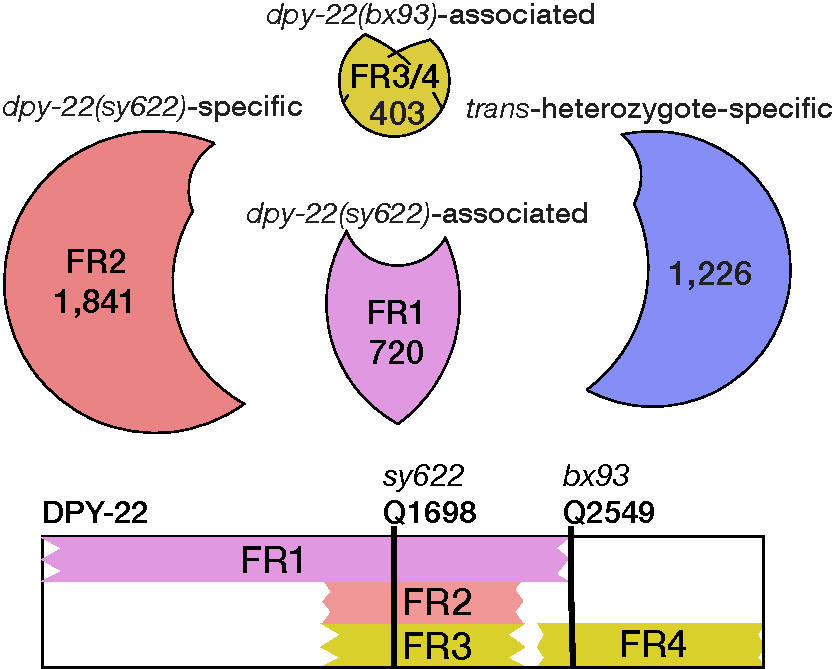
\includegraphics[width=0.5\textwidth]{../figs/inferred_domains.pdf}
  \caption{
    The modules associated with each phenotypic class can be
    mapped to intragenic locations. The beginning and end positions of
    these functions are unknown,
    so edges are drawn as ragged lines. Thick horizontal lines show the
    limit where each function could end, if known. We postulate that the
    \emph{bx93}-associated function exists as two distinct modules in the tail
    region of this gene. Some of the modules shown may represent the same
    structures. Future experiments are required to make a complete determination
    of the number and nature of these modules.
  }
\label{fig:domains}
\end{figure}


\subsection*{Statistical artifacts associated with this analysis}
Transcriptomic phenotypes generate large amounts of information that can be used
to accurately determine molecular structures. However, due to the large number of
tests performed, false positive and false negative events occur frequently enough
to create populations of transcripts that have anomalous behaviors. It is
necessary to identify what modules or populations are most at risk of these events
and to what extent these modules may be polluted by false signals to prevent
over-interpretation. In our experiment, we can identify two populations that are
most at risk for statistical artifacts.

The \emph{sy622}-associated class and the \emph{bx93}-associated class are
presented in our analysis as independent modules. A transcript that is
differentially expressed in both \emph{sy622} homozygotes and \emph{trans}-heterozygotes
is assigned to the \emph{sy622}-associated class if and only if it is not
differentially expressed in \emph{bx93} homozygotes. If a transcript is falsely
found to have wild-type expression in \emph{bx93} homozygotes, then this transcript
will be misclassified, and it will contribute signal to the \emph{sy622}-associated
class. Assuming a false negative
rate of 10\%, the number of transcripts that are mis-classified in this manner
is approximately 34 (10\% of 339 genes differentially expressed in \emph{bx93}
homozygotes). This constitutes almost 5\% of the signal in the \emph{sy622}-associated
class. On the other hand, a transcript could be misclassified in the
\emph{bx93}-associated class in several ways. We enumerate the most likely
events next. First, an \emph{sy622}-associated transcript could be called as
differentially expressed in \emph{bx93} homozygotes. This event would contribute
$\sim 19$ genes (10\% of 193 genes differentially expressed in all genotypes) to
the \emph{bx93}-associated class. Second, a transcript in the \emph{sy622}-associated
class could be falsely identified as differentially expressed in \emph{bx93}
homozygotes. This would be expected to contribute 5 transcripts. A similar event
would also contribute 5 transcripts if the misclassification occurred in
\emph{trans}-heterozygotes. Therefore, we might expect that 29 transcripts are
falsely contributing to the \emph{bx93}-associated class, which constitutes
$\sim 10\%$ of the total signal. Therefore, the \emph{bx93}-associated class is
twice as vulnerable to statistical artifacts as the \emph{sy622}-associated class.
Moreover, most of the signal comes from transcripts that should have been classified
in the \emph{sy622}-associated class. Therefore, statistical noise will tend
to make these two classes appear more similar than they really are. Fortunately,
since both classes contained hundreds of genes and statistical contamination
was less than 20\%, our signal/noise ratio is able to resolve differences in the
behaviors of these populations without trouble.

The phenotypic class that is most likely to be artifactual is the \emph{bx93}-specific
class. This class contains 43 genes. The expected number of transcripts that
are falsely assigned as differentially expressed in \emph{bx93} homozygotes is
33. The probability that such a false positive appears in any other genotype is
approximately 20\% (3,000 genes identified between the two other genotypes divided
by 21,0000 the total number of genes that were successfully sequenced). Thus,
the \emph{bx93}-specific class on average contains 26 genes (80\% of 33) that
are false positives. False negative rates will also contribute to the
\emph{bx93}-specific class by moving genes from the \emph{bx93}-associated class
into the \emph{bx93}-specific class. Such misassignments are expected to
contribute $\sim 11$ transcripts assuming a 10\% false negative rate. In total,
we estimate 37/43 genes in the \emph{bx93}-specific class can be explained by
sources of statistical artifacts, leading us to conclude that this phenotypic
class does not exist and is simply the result of statistical noise.

\subsection*{The \emph{trans}-heterozygote specific phenotypic class is not a
             statistical artifact}
In our study, we found a large class of transcripts that were exclusively
differentially expressed in \emph{trans}-heterozygotes. The size of this class
makes a statistical artifact unlikely. As a result, this class must be understood
as either a legitimate aspect of \dpy{} biology, reflecting antagonistic
dosage-responsive tissue-specific effects, or as a strain-specific artifact.
The genotype of the
heterozygote includes a mutation at the \gene{dpy-6} locus which acts as a balancer
for the
\emph{bx93} mutation. One possibility is that the \emph{dpy-6} loss-of-function
mutation is not recessive for transcriptomic phenotypes and is responsible for
the dysregulation of the new genes observed in the heterozygote. Another
possibility is that the \emph{dpy-6} strain had eQTLs that are affecting gene
expression levels in a complex manner. As the cost of sequencing becomes
lower, and with improved genetic engineering tools that allow the creation of
background-free mutations, it will become increasingly important to rule out
these hypotheses by sequencing additional independently derived identical
alleles.

\subsection*{Transcriptomic genetics}
Allelic series are a cornerstone of genetic analyses. Classically, these series
have been important to understand multiple aspects of a gene by comparing and
contrasting the properties of different alleles in homozygotes as well as
heterozygotes. Due to their sensitivity and quantitative nature, transcriptomic
phenotypes represent an exciting new phenotype with which to study these series.
Here, we have shown that transcriptomic phenotypes can quickly and easily
partition gene sets into phenotypic classes that have different statistical and
physiological properties with minimal bioinformatic complexity. Expression
profiles can be used for genetic pathway analysis~\cite{Dixit2016} as well as
for the identification of novel cellular or animal
states~\cite{Angeles-Albores2017,Villani2017}. In addition to sequencing
various cell types to understand cellular diversity, we should sequence diverse
alleles to understand genotype-genotype variation.

\section*{Methods}
\label{sec:methods}
\subsection*{Strains used}
Strains used were N2 wild-type (Bristol),
PS4087 \gene{dpy-22(sy622)},
PS4187 \gene{dpy-22(bx93)},
%line break inserted below because \gene{...} doesn't linebreak well
and PS4176\\ \gene{dpy-6(e14) dpy-22(bx93)/ + dpy-22(sy622)}.
% MT4866 \gene{let-60(n2021)}, and
% MT2124 \gene{let-60(n1046gf)}.
All lines were grown on standard nematode growth media (NGM) Petri plates seeded
with OP50 \ecol{} at 20\degree{}C~\cite{Brenner1974}.

\subsection*{Strain synchronization, harvesting and RNA sequencing}
All strains were synchronized by bleaching
P$_0$'s into virgin S. basal (no cholesterol or ethanol added) for 8--12 hours.
Arrested L1 larvae were placed in NGM plates seeded with OP50 at 20\degree{}C
and allowed to grow to the young adult stage (as assessed by vulval morphology
and lack of  embryos). RNA extraction was performed as described in~\cite{} and
sequenced using a previously described protocol~\cite{Angeles-Albores2017}.

\subsection*{Read pseudo-alignment and differential expression}
Reads were pseudo-aligned to the \cel{} genome (WBcel235) using
Kallisto~\cite{Bray2016}, using 200 bootstraps and with the sequence bias
(\texttt{--seqBias}) flag. The fragment size for all libraries was set to 200
and the standard deviation to 40. Quality control was performed on a subset of
the reads using FastQC, RNAseQC, BowTie and
MultiQC~\cite{Andrews2010,Deluca2012,Langmead2009,Ewels2016}. All libraries had
good quality scores.

Differential expression analysis was performed using
Sleuth~\cite{Pimentel2016a}. Briefly, we used a general linear model to identify
genes that were differentially expressed between wild-type and mutant libraries.
To increase our statistical power, we pooled wild-type replicates from other
published~\cite{} and unpublished analysis. All wild-type replicates were
collected at the same stage (young adult). In total, we had 10 wild-type
replicates from 4 different batches, which heightened our statistical
power. To account for batch effects, we added a batch correction term to our
general linear model.

\subsection*{Non-parametric bootstrap}
We performed non-parametric bootstrap testing to identify whether two
distributions had the same mean. Briefly, the two datasets were mixed, and
samples were selected at random with replacement from the mixed population into
two new datasets. We calculated the difference in the means of these new
datasets. We iterated this process $10^6$ times. To calculate a $p$-value that the
null hypothesis is true, we identified the number of times a difference in the
means of the simulated populations was greater than or equal to the observed
difference in the means of the real population. We divided this result by $10^6$
to complete the calculation for a $p$-value. If an event where the difference in
the simulated means was greater than the observed difference in the means was
not observed, we reported the $p$-value as $p<10^{-5}$. Otherwise, we reported the
exact $p$-value. We chose to reject the null hypothesis that the means of the two
datasets are equal to each other if $p < 0.05$.

\subsection*{Dominance analysis}
\label{subsec:dominance}
We modeled allelic dominance as a weighted average of allelic activity. Briefly,
our model proposed that $\beta$ coefficients of the heterozygote,
$\beta_{a/b,i,\text{Pred}}$, could be modeled as a linear combination of the
coefficients of each homozygote:
\begin{equation}
  \beta_{a/b,i,\text{Pred}}(d_a) = d_a\cdot \beta_{a/a,i} + (1-d_a)\cdot \beta_{b/b,i},
\end{equation}
where $\beta_{k/k, i}$ refers to the $\beta$ value of the $i$th isoform in a
genotype $k/k$, and $d_a$ is the dominance coefficient for allele $a$.

To find the parameters $d_a$ that maximized the probability of observing the
data, we found the parameter, $d_a$, that maximized the equation:
\begin{equation}
    P(d_a|D,H,I) = \prod_{i \in S}\frac{1}{\sqrt{2\pi \sigma_i^2}}
                   \exp{\frac{{(\beta_{a/b,i,\text{Obs}} -
                                \beta_{a/b,i,\text{Pred}}(d_a))}^2}{
                                2\sigma_i^2}}
\end{equation}
where $\beta_{a/b,i,\text{Obs}}$ was the coefficient associated with the $i$th
isoform in the \emph{trans}-het $a/b$ and $\sigma_i$ was the standard error of the
$i$th isoform in the \emph{trans}-heterozygote samples as output by Kallisto. $S$ is
the set of isoforms that participate in the regression (see main text). This
equation describes a linear regression which was solved numerically.

\subsection*{Code}
All code was written in Jupyter notebooks~\cite{Perez2007} using the Python
programming language. The Numpy, pandas and scipy libraries were used for
computation~\cite{VanDerWalt2011,McKinney2011,Oliphant2007} and the matplotlib
and seaborn libraries were used for data visualization~\cite{Hunter2007,Waskom}.
Enrichment analyses were performed using the WormBase Enrichment
Suite~\cite{Angeles-Albores2016}. For all enrichment analyses, a $q$-value of
less than $10^-3$ was considered statistically significant. For gene ontology
enrichment analysis, terms were considered statistically significant only if they
also showed an enrichment fold-change greater than 2.

\section*{Acknowledgements}
This work was supported by HHMI with whom PWS is an investigator and by the
Millard and Muriel Jacobs Genetics and Genomics Laboratory at California
Institute of Technology. All strains were provided by the CGC, which is funded
by NIH Office of Research Infrastructure Programs (P40 OD010440). This article
would not be possible without help from Dr.\ Igor Antoshechkin and Dr.\ Vijaya
Kumar who performed the library preparation and sequencing.

%This is where your bibliography is generated.
\bibliography{citations}
\bibliographystyle{naturemag}

\end{document}
